Le componenti che invece si è deciso di andare a sviluppare durante la seconda iterazione sono: 
\begin{itemize}
	\item \textbf{Componente \textit{Automatic Book registration:}} la componente \textit{Automatic Book registration} fa riferimento all’ UC10
	(~\ref{itemize:UC10} )
	(figlio del caso d'uso più generico UC5 
	(~\ref{itemize:UC5} );
	questa funzionalità consente di ottenere, in maniera del tutto automatica, le informazioni necessarie per registrare uno specifico libro all'interno della piattaforma di book crossing. La componente si presenta nel seguente modo:
	\begin{itemize}
		\item \textit{GUI:} interfaccia grafica utilizzata per registrare un libro, in maniera automatica, nella rete di Book Crossing. Verranno quindi messe a disposizione una serie di interfaccie grafiche, le quali permetteranno di scansionare il codice ISBN del libro deisderato, unitamente ad una parte GUI utilizzata per mostrare le informazioni relative al libro che è appena stato scansionato.
		\item \textit{Model:} si fa carico di ricevere le informazioni relative al libro e, sfruttando la parte Data, restituisce alla parte GUI il BCID con il quale siglare il libro;
		\item \textit{Data:} le informazioni relative al libro che si vuole aggiungere sono memorizzate nel Database RDS, associandolo all'utente che attualmente lo possiede. 
	\end{itemize}
	\item \textbf{Componente \textit{Login:}}  la componente \textit{Login} fa riferimento all’ UC13 
	(~\ref{itemize:UC13} )
	, ovvero alla funzione che permette ad un utilizzatore dell'applicazione di loggarsi all'interno della piattaforma di Book Crossing, potendo così effettuare operazioni di suo interesse sui testi disponibili.
	La componente si presenta nel seguente modo:
	\begin{itemize}
		\item \textit{GUI:} interfaccia grafica, composta da due caselle di testo, le quali devono essere riempite con username e password, unitamente ad un pulsante che permette di iniviare la richiesta/verifica di login corretto. Per chi non fosse già registrato, è fornita la possibilità di iscriversi alla piattaforma (questo però rappresenta un caso d'uso separato);
		\item \textit{Model:} si fa carico di verificare la coerenza dei dati inseriti tramite il componente grafico, restituendo l'esito a chi ha appena tentato di effettuare il login.
		\item \textit{Data:} le informazioni relative all'utente che sta tentando di loggarsi.
	\end{itemize}
	\item \textbf{Componente \textit{Book reservation:}}  La componente \textit{Book reservation} fa riferimento all’ U13 (~\ref{itemize:UC13} ), ovvero alla funzione di prenotazione di un libro, la quale richiede prima un'operazione di ricerca dello stesso all'interno della community e poi, se possibile, permette di effettuare la prenotazione  effettiva. La componente si presenta nel seguente modo:
	\begin{itemize}
		\item \textit{GUI:} interfaccia grafica utilizzata per poter procedere con la prenotazione di un libro della rete di Book Crossing. In questo caso sarà possibile compiere tale azione attraverso una procedura di ricerca del libro, oppure navigando nella propria sezione personale del profilo;
		\item \textit{Model:} si fa carico di gestire la coda relativa alla prenotazione di un determinato libro, in modo da poterle soddisfare. La gestione e la computazione della prenotazione è affidata ad un algoritmo il quale va ad appoggiarsi alla parte Data per poter risalire ai dati dei richiedenti;
		\item \textit{Data:} le informazioni relative al libro che si vuole prenotare e agli utenti richiedenti le quali sono memorizzate nel Database.
	\end{itemize}
\end{itemize}
Partendo dalla figura \ref{fig:Diagramma della class ComputeRequest} relativa a quanto sviluppato nella precedente iterazione, possiamo andare ad osservare come, nella successiva immagine, il medesimo diagramma delle classi si completa nel seguente modo:
\begin{figure}[h]
	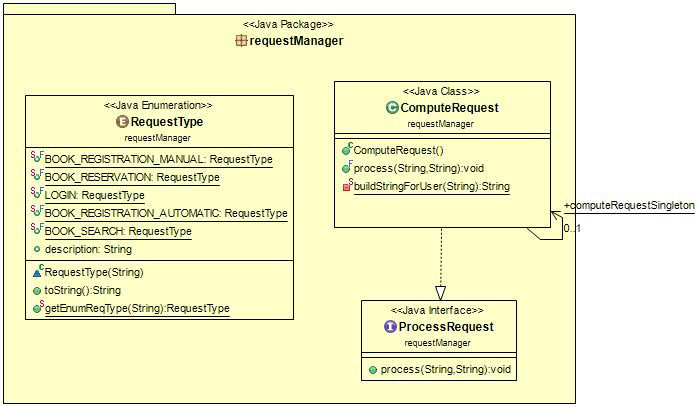
\includegraphics[width=\textwidth]{Immagini/UML_ComputeRequestServer2}
	\caption{Diagramma della classe ComputeRequest}
	\label{fig:Diagramma della class ComputeRequest2}
\end{figure}
\\ \noindent
Si può notare infatti come alla \textbf{\textit{RequestType}} si aggiungano 3 casi in più, relativi proprio ai nuovi componenti sviluppati in questa seconda iterazione. Allo stesso modo anche il codice si completa così
\begin{lstlisting}[caption={Tipologia di richieste aggiuntive gestite durante la seconda iterazione},captionpos=b]
case BOOK_RESERVATION:
	boolean rs = book.reserve(username);
	Communication.getInstance().send(username, "requestType:1;result:" + (rs?1:0));
	break;
case LOGIN:
	Communication.getInstance().send(username, "requestType:2;result:" + "Success" + ";" + buildStringForUser(username));
	break;
case BOOK_REGISTRATION_AUTOMATIC:
	result = b.insert();
	Communication.getInstance().send(username, "requestType:4;result:" + (result?1:0) + ";BCID:" + b.getBCID());
	break;
\end{lstlisting}

Questo si va ad aggiungere a quanto sviluppato nella prima iterazione: a questo punto possiamo quindi gestire le richieste del client compilate nel formato descritto relative ai componenti disponibili nella prima e seconda iterazione.